\chapter{Conception}
\label{chap:conception}

\section{Introduction}

Ce chapitre se concentre sur la conception de l'application de conversion de wireframes dessinées à la main en interfaces web. Nous aborderons la conception générale, en discutant des choix d'architecture physique et logique. Ensuite, nous passerons à la conception détaillée, en présentant des diagrammes de séquence et de classes pour illustrer le fonctionnement de l'application. Enfin, nous explorerons la conception de la base de données pour stocker les données nécessaires au processus de conversion.

\section{Conception générale}

\subsection{Choix de l'architecture physique}

mezelt makhdemthech

\subsection{Choix de l'architecture logique}

En ce qui concerne l'architecture logique, nous optons pour une architecture MVC (Modèle-Vue-Contrôleur) pour organiser notre code de manière modulaire et faciliter la maintenance et l'extension de l'application. Le modèle représentera les données et la logique métier, la vue sera responsable de l'interface utilisateur, tandis que le contrôleur gérera les interactions entre le modèle et la vue.
\begin{figure}[h]
    \centering
    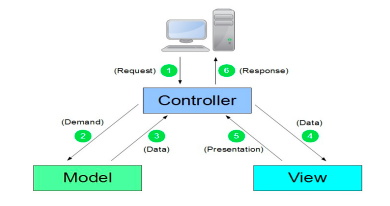
\includegraphics[width=\textwidth]{images/mvc.png}
    \caption{Illustration de l'architecture MVC}
    \label{fig:mvc_architecture}
\end{figure}
\vspace{3cm}
\newline Comme indiqué dans la figure 3.1 on peut distinguer trois couches différentes [R15] :
\newline— Modèle : c’est la partie qui exécute la logique métier c’est à dire la récupération
des données;
\newline— Vue : cette couche permet de produire une présentation des données venant du
modèle;
\newline— Contrôleur : cette couche responsable de gérer les requêtes et de coordonner les
taches à exécuter entre Vue et Modèle.

\section{Conception Détaillée}

\subsection{Diagrammes de séquence}

Les diagrammes de séquence sont des outils essentiels pour décrire l'interaction entre les différents composants de notre système. Ils permettent de visualiser le flux de contrôle lors de l'exécution des fonctionnalités de l'application. Nous présenterons plusieurs diagrammes de séquence pour illustrer le processus de conversion des wireframes en interfaces web.


\begin{figure}[H]
    \centering
    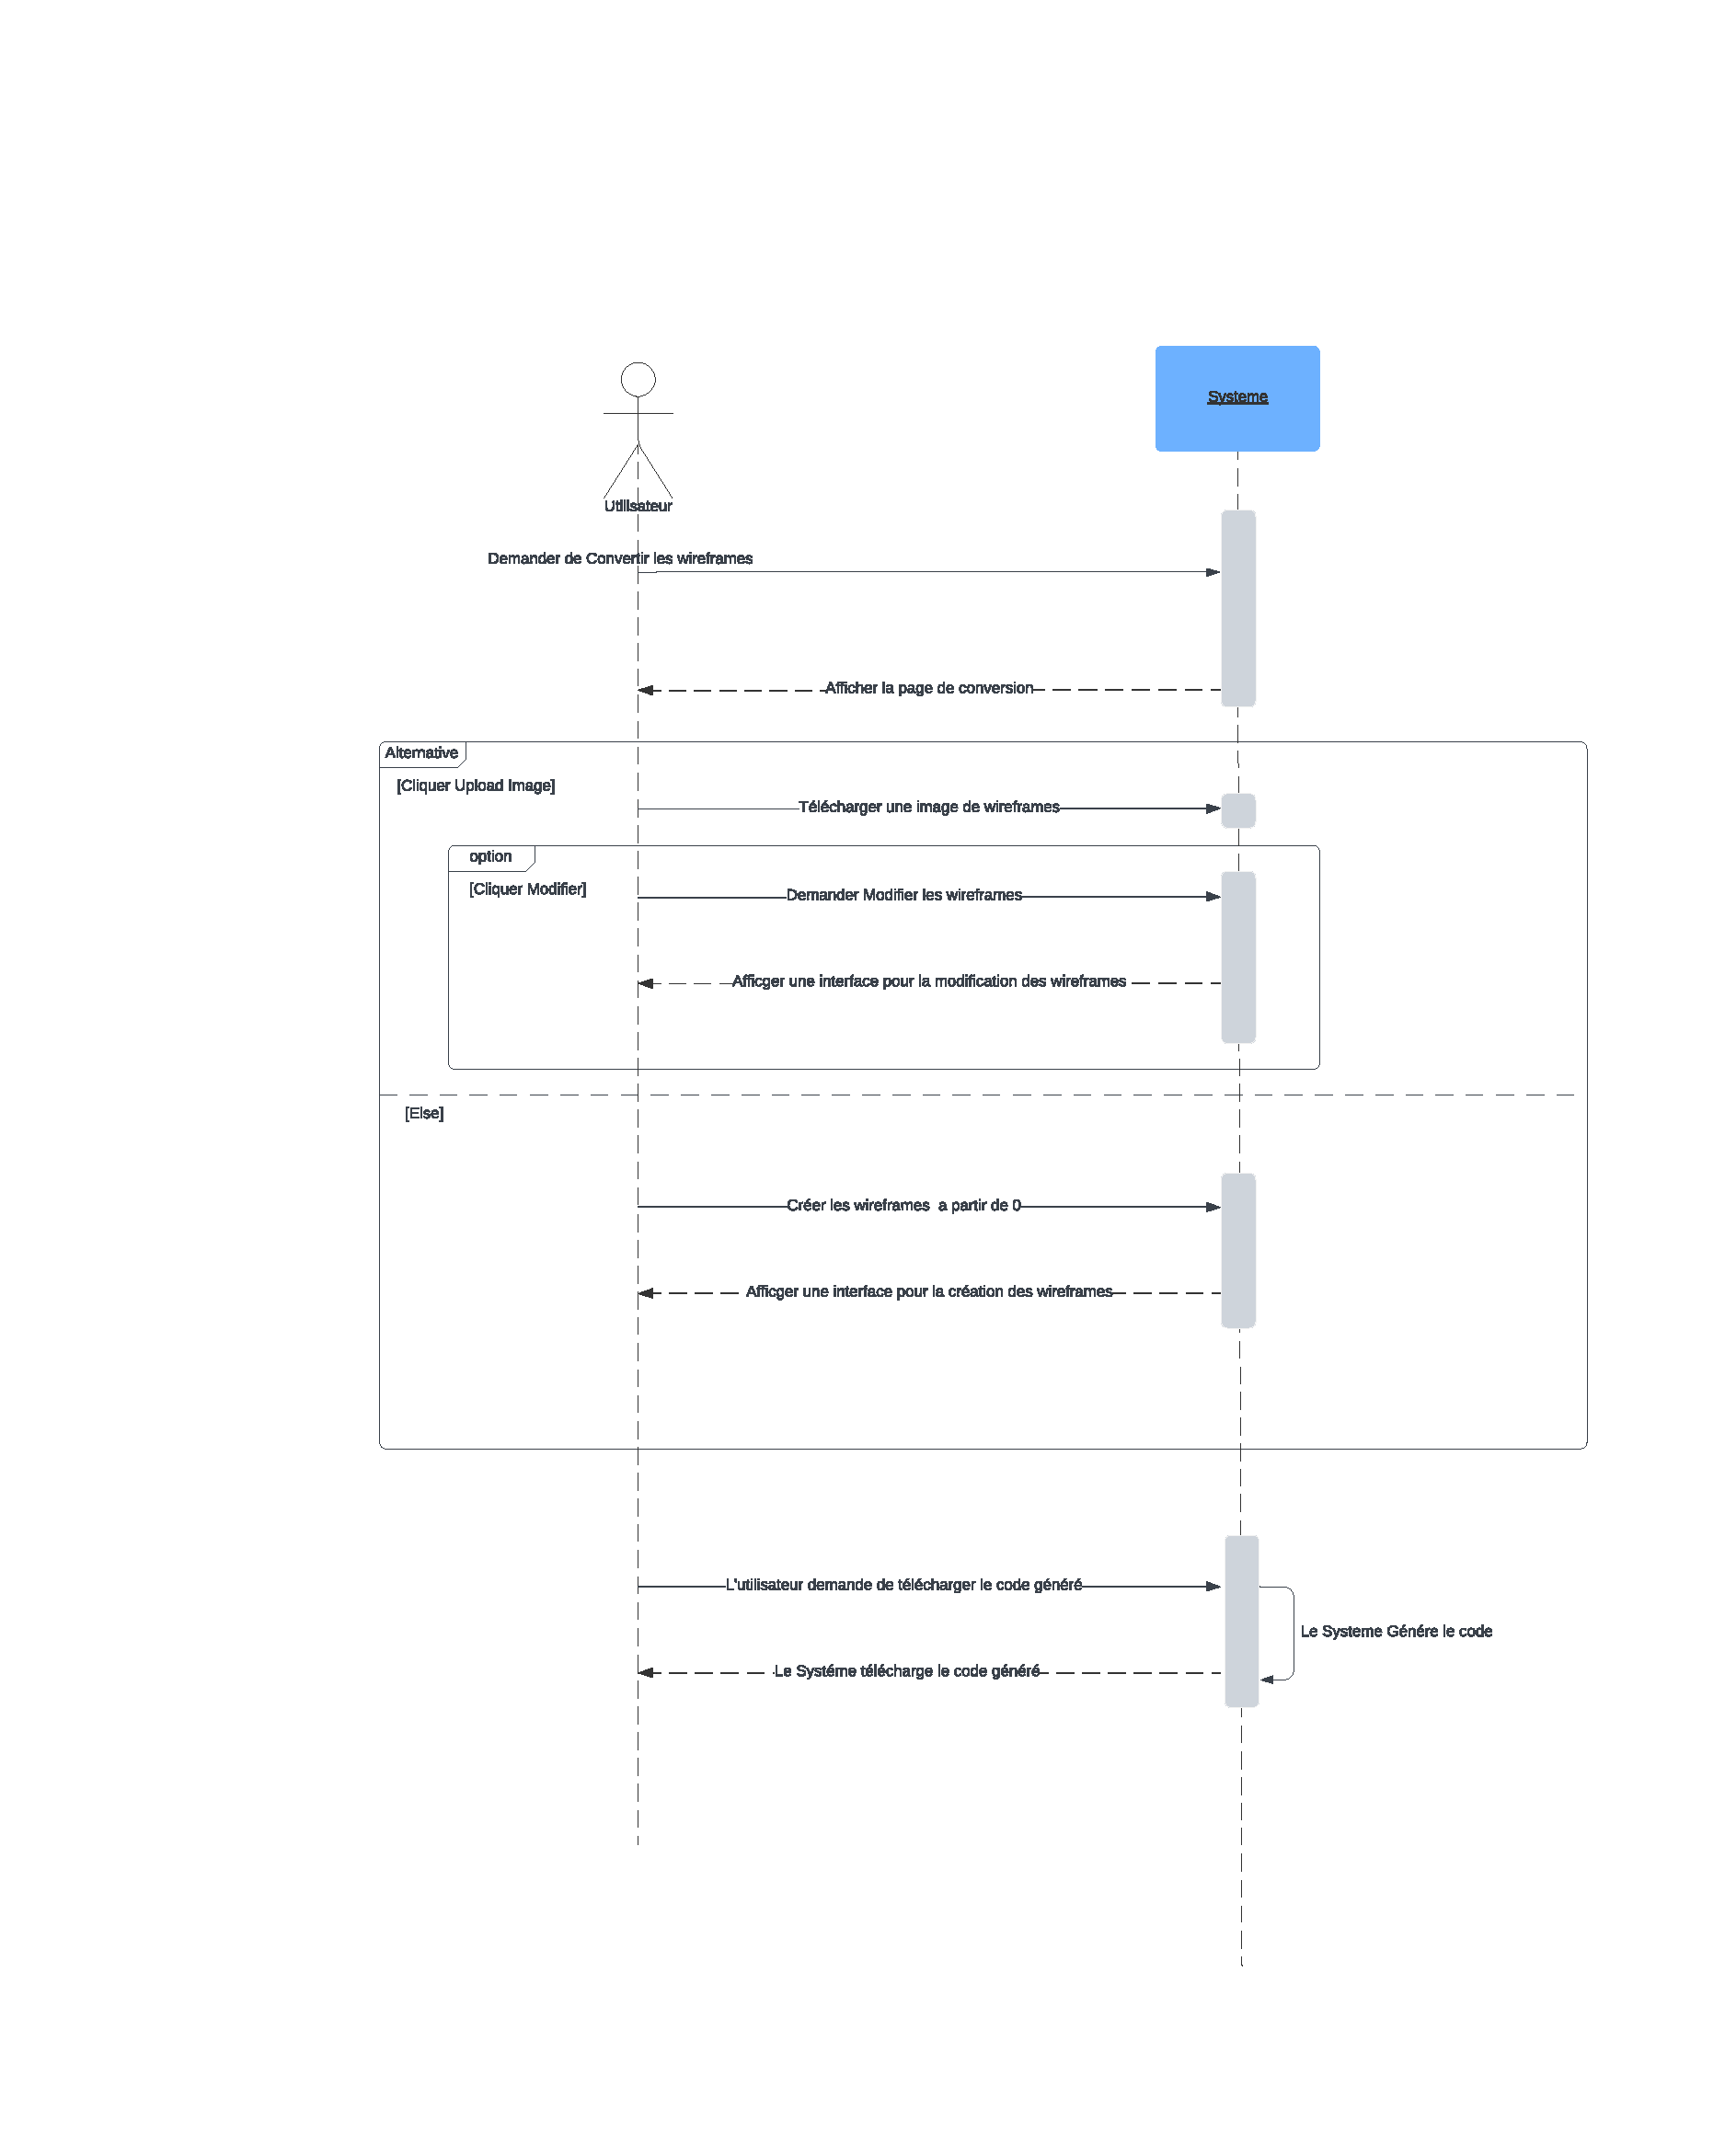
\includegraphics[width=0.5\linewidth]{images/Sequence diagram1 (2).pdf}
    \caption{Diagramme de séquence pour la conversion de wireframes en code avec téléchargement}
    \label{fig:sequence_diagram_download}
\end{figure}
\subsection{Diagrammes de classes}

Les diagrammes de classes représentent la structure statique de notre système, en identifiant les classes, les attributs et les relations entre elles. Nous utiliserons des diagrammes de classes pour modéliser les différents composants de notre application, y compris les modèles de données, les contrôleurs et les vues.

\section{Conception de base des données}

La conception de la base de données est une étape cruciale pour assurer la persistance des données de notre application. Nous utiliserons un système de gestion de base de données relationnelle tel que MySQL ou PostgreSQL pour stocker les wireframes importées, les codes générés et d'autres informations pertinentes. Nous élaborerons un schéma de base de données normalisé pour garantir l'intégrité et la cohérence des données.

\section{Conclusion}

Ce chapitre a présenté la conception de notre application de conversion de wireframes en interfaces web. Nous avons discuté des choix d'architecture physique et logique, puis avons exploré la conception détaillée à l'aide de diagrammes de séquence et de classes. Enfin, nous avons abordé la conception de la base de données pour stocker les données nécessaires au fonctionnement de l'application. Cette conception fournira une base solide pour le développement de l'application et assurera son efficacité et sa fiabilité.
